\section{Spherical and Cylindrical Coordinates}

\begin{outcome}
\begin{enumerate}
\item[A.]  Understand cylindrical and spherical coordinates.

\item[B.]  Convert points between Cartesian, cylindrical, and spherical coordinates.
\end{enumerate}
\end{outcome}

Spherical and cylindrical coordinates are two generalizations of polar coordinates to three dimensions. We will first look at \textbf{cylindrical coordinates} \index{cylindrical coordinates}.

When moving from polar coordinates in two dimensions to cylindrical coordinates in three dimensions, we use the polar coordinates in the $xy$
plane and add a $z$ coordinate. For this reason, we use the notation $(r, \theta, z)$ to express cylindrical coordinates.
The relationship between Cartesian coordinates $(x,y,z)$ and cylindrical coordinates $(r, \theta, z)$ is given by  
\begin{align*}
x& =r\cos \left( \theta \right)  \\
y& =r\sin \left( \theta \right)  \\
z& =z
\end{align*}
where $r\geq 0$, $\theta \in \lbrack 0,2\pi ),$ and $z$ is simply the Cartesian
coordinate. Notice that $x$ and $y$ are defined as the usual polar coordinates in the $xy$-plane. Recall that $r$ is defined as the length of the ray from the origin to the point $(x,y,0)$, while $\theta$ is the angle between the positive $x$-axis and this same ray. 

To illustrate this coordinate system, consider the following two pictures.
In the first of these, both $r$ and $z$ are known. The cylinder corresponds to a given value for $r$. A useful way to think of $r$ is
as the distance between a point in three dimensions and the $z$-axis. Every point on the cylinder shown is at the same distance from the $z$-axis. Giving a value for $z$ results in a horizontal circle, or cross section of the cylinder at the given height on the $z$ axis (shown below as a black line on the cylinder). In the second picture, the point is specified completely by also knowing $\theta$ as shown.

\begin{center}
\begin{tikzpicture}
\node at (-5, 2.5){$z$};
\node at (-2.5, -2){$y$};
\node at (-7.5, -2){$x$};
\node at (-5,0){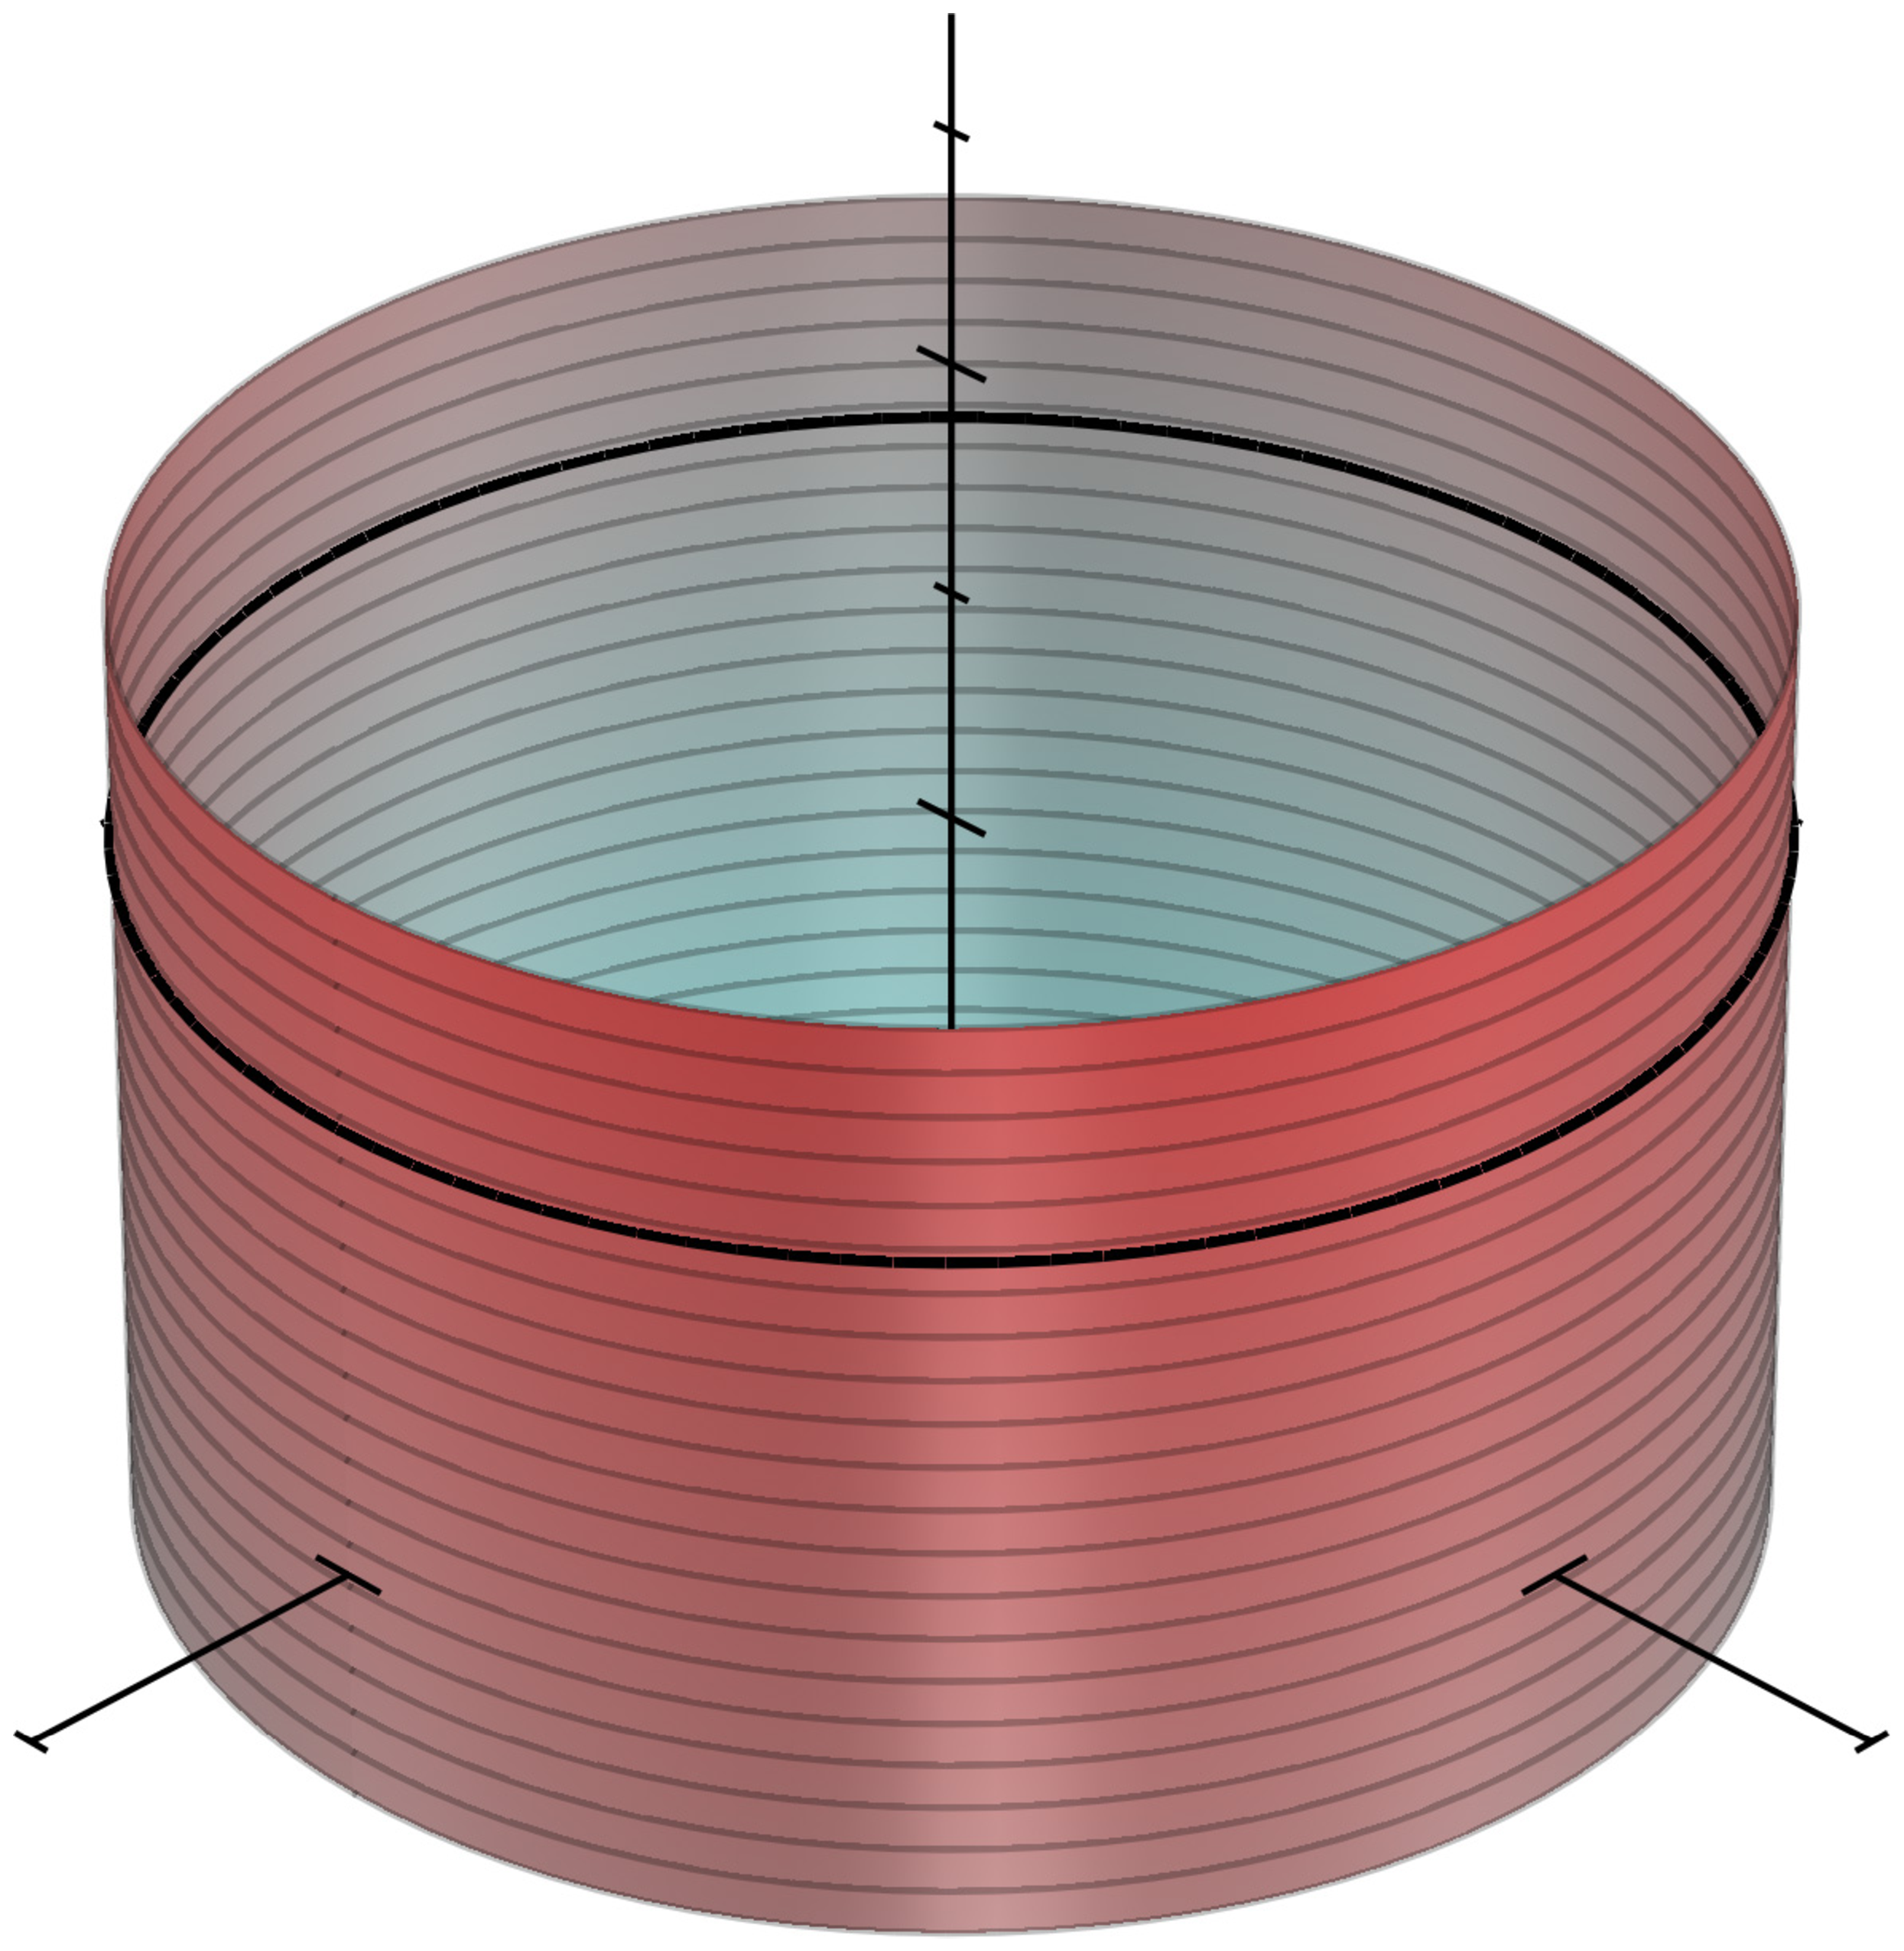
\includegraphics[width=.25\textwidth]{figures/cylinder.eps}};
\node at (-5,-3){$r$ and $z$ are known};
\draw(-1,-1,0)--(3,-1,0);
\draw(1,-1,0)--(1,2,0);
\draw[dotted](1,-1,-2)--(1,-1,0);
\draw(1,-1,0)--(1,-1,2);
\draw(1,1,0) circle [x radius=1.5cm, y radius=0.5cm];
%\draw[red](1,-1,0)--(1.5,0.55,0);
\draw[fill, red](1.5,0.55,0) circle [radius=2pt];
\draw[blue](1,-1,0)--(1.5,-1.5,0);
\draw[fill,blue](1.5,-1.5,0) circle [radius=2pt];
\draw[red](1.5,0.55,0)--(1.5,-1.5,0);
\draw[purple, dotted](1.5,0.55,0)--(1,0.65,0);
\draw[fill,purple](1,0.65,0) circle [radius=2pt];
\node[below right] at (1.5,0.55,0){$(x,y,z)$};
\node[right] at (1.5,-1.5,0){$(x,y,0)$};
\node[below] at (1,-1.2,0){$\theta$};
\node[right] at (3,-1,0){$y$};
\node[above] at (1,2,0){$z$};
\node[below] at (1,-1,2){$x$};
\node[above] at (1.4,-1,0){$r$};
\node[left] at (1,0.65,0){$z$};
\node at (1, -3){$r$, $\theta$ and $z$ are known};
\end{tikzpicture}
\end{center}

 Every point of three dimensional
space other than the $z$ axis  has  unique cylindrical coordinates. Of course there are infinitely many cylindrical coordinates for the
origin and for the $z$-axis. Any $\theta $ will work if $r=0$ and $z$ is given.  

Consider now \index{spherical coordinates} \textbf{spherical coordinates}, the second generalization of polar form in three dimensions. For a point $(x,y,z)$ in three dimensional space, the spherical coordinates are defined as follows.
\begin{equation*}
\begin{array}{l}
\rho: \mbox{the length of the ray from the origin to the point}\\
\theta: \mbox{the angle between the positive $x$-axis and the ray from the origin to the point $(x,y,0)$}\\
\phi: \mbox{the angle between the positive $z$-axis and the ray from the origin to the point of interest}
\end{array}
\end{equation*}
The spherical coordinates are determined by $\left( \rho ,\phi
,\theta \right) $. The relation between these and the Cartesian coordinates $\left( x,y,z \right)$ for a point
are as follows.  
\begin{align*}
x& =\rho \sin \left( \phi \right) \cos \left( \theta \right) ,\ \phi \in 
\left[ 0,\pi \right]  \\
y& =\rho \sin \left( \phi \right) \sin \left( \theta \right) ,\text{ }\theta
\in \lbrack 0,2\pi ) \\
z& =\rho \cos \phi \text{, }\rho \geq 0.
\end{align*}

Consider the pictures below. The first illustrates the surface when $\rho$ is known, which is a sphere of radius $\rho$. The second picture corresponds to knowing both $\rho $ and $\phi$, which results in a circle about the $z$-axis. Suppose the first picture demonstrates a graph of the Earth. Then the circle in the second picture would
correspond to a particular latitude. 

\begin{center}
\begin{tikzpicture}
\node at (-6, 2.5){$z$};
\node at (-3.5, -1){$y$};
\node at (-8.5, -1.5){$x$};
\node at (-6,0){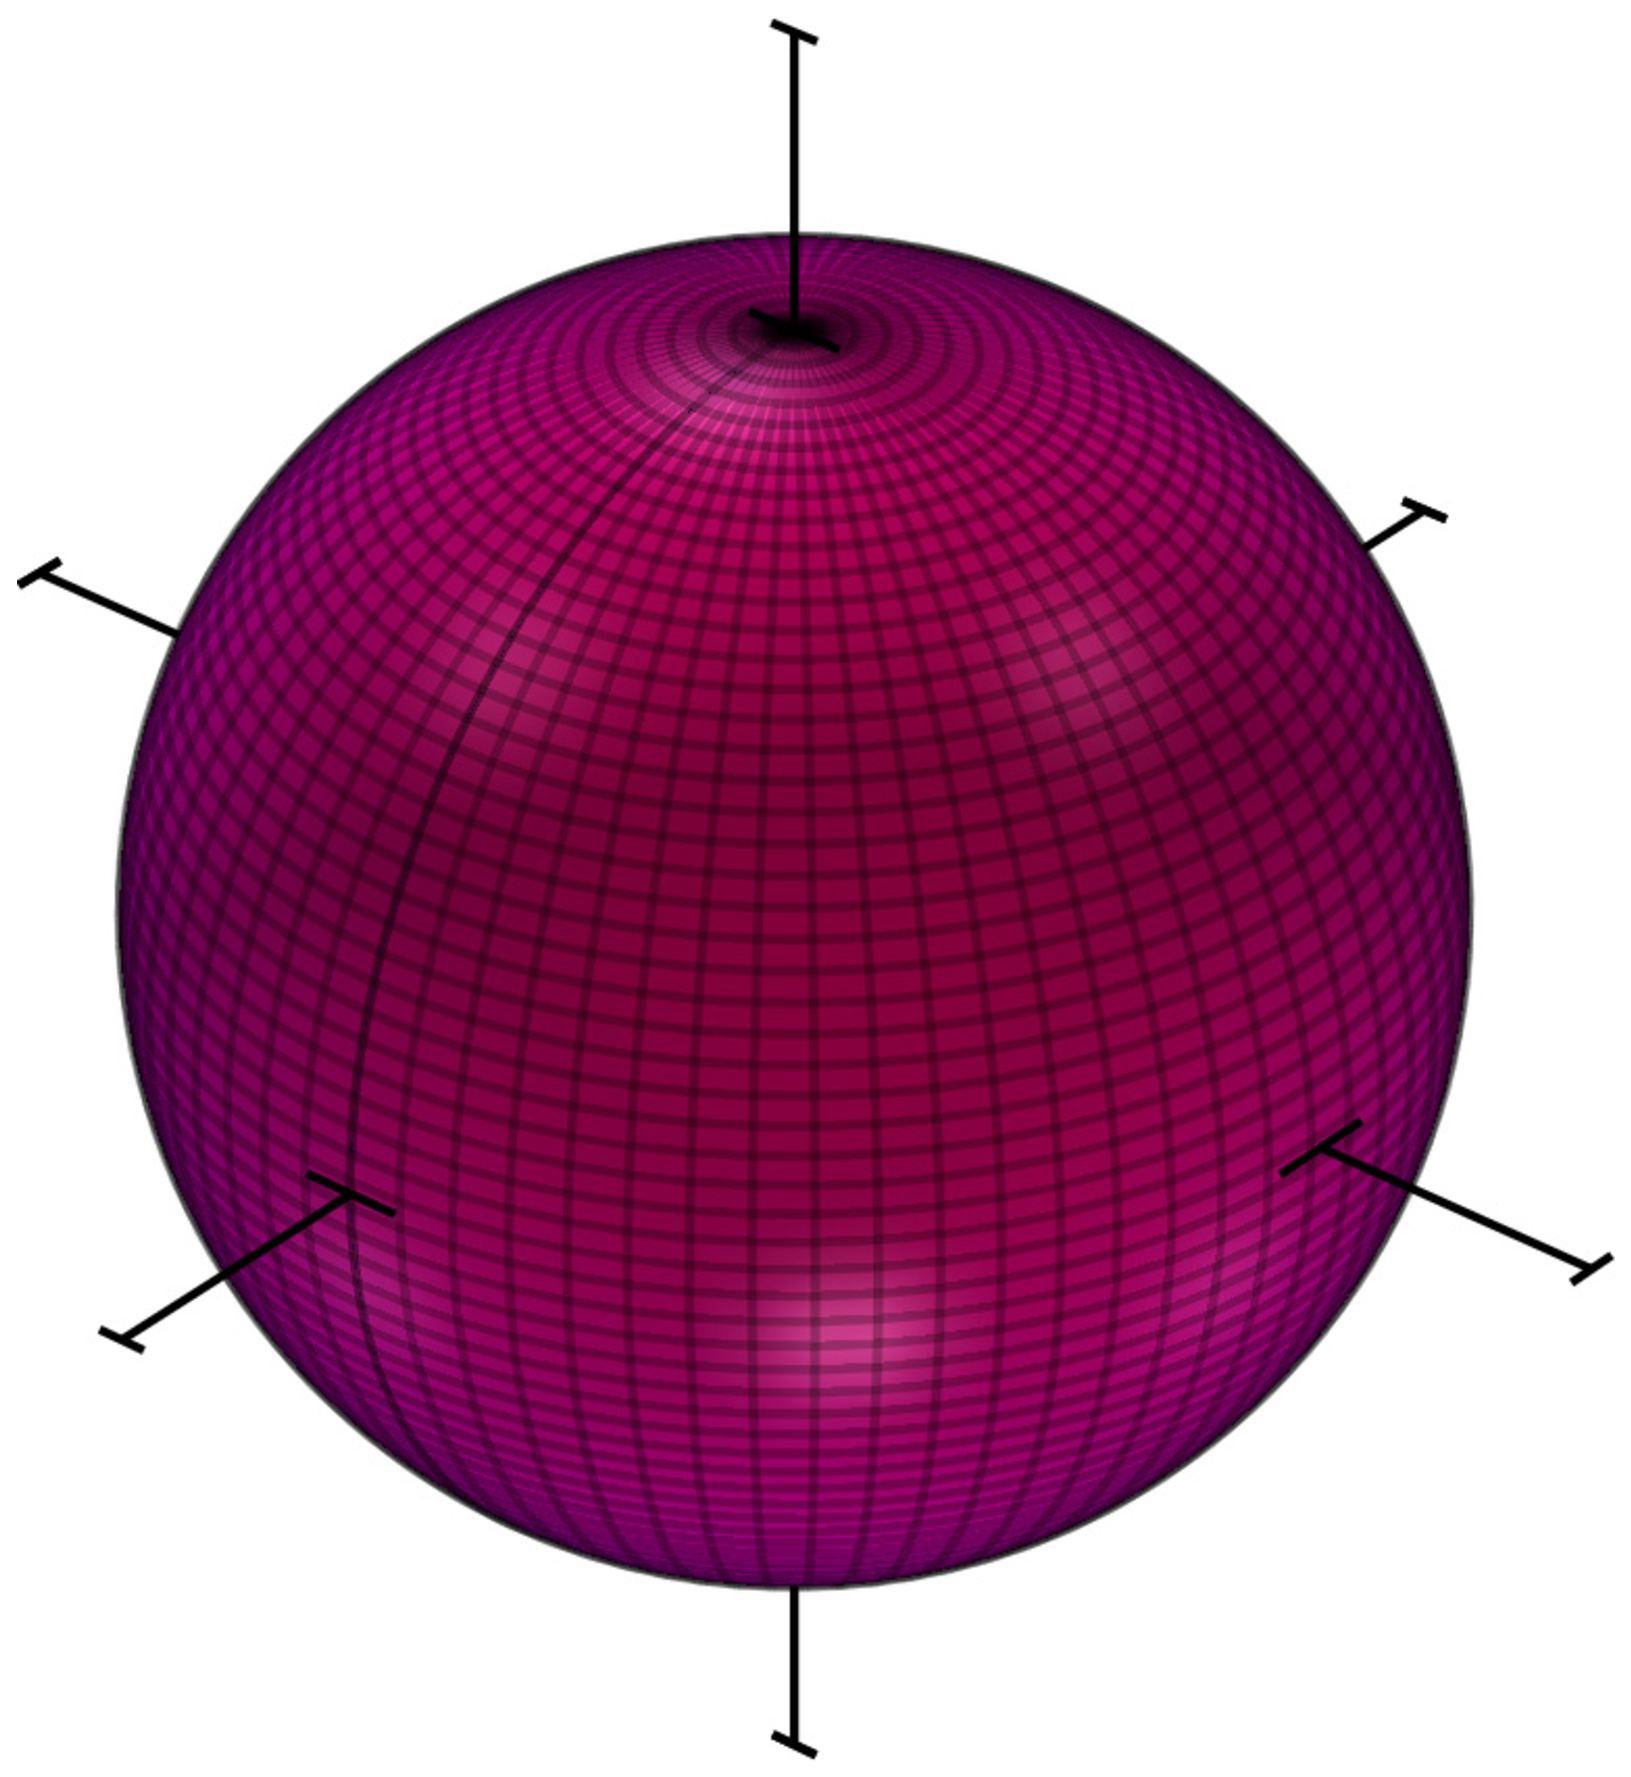
\includegraphics[width=.25\textwidth]{figures/sphericalcoordinates.eps}};
\node at (-6,-3){$\rho$ is known};
\node at (2,-3){$\rho$ and $\phi$ are known};
\node at (2,0){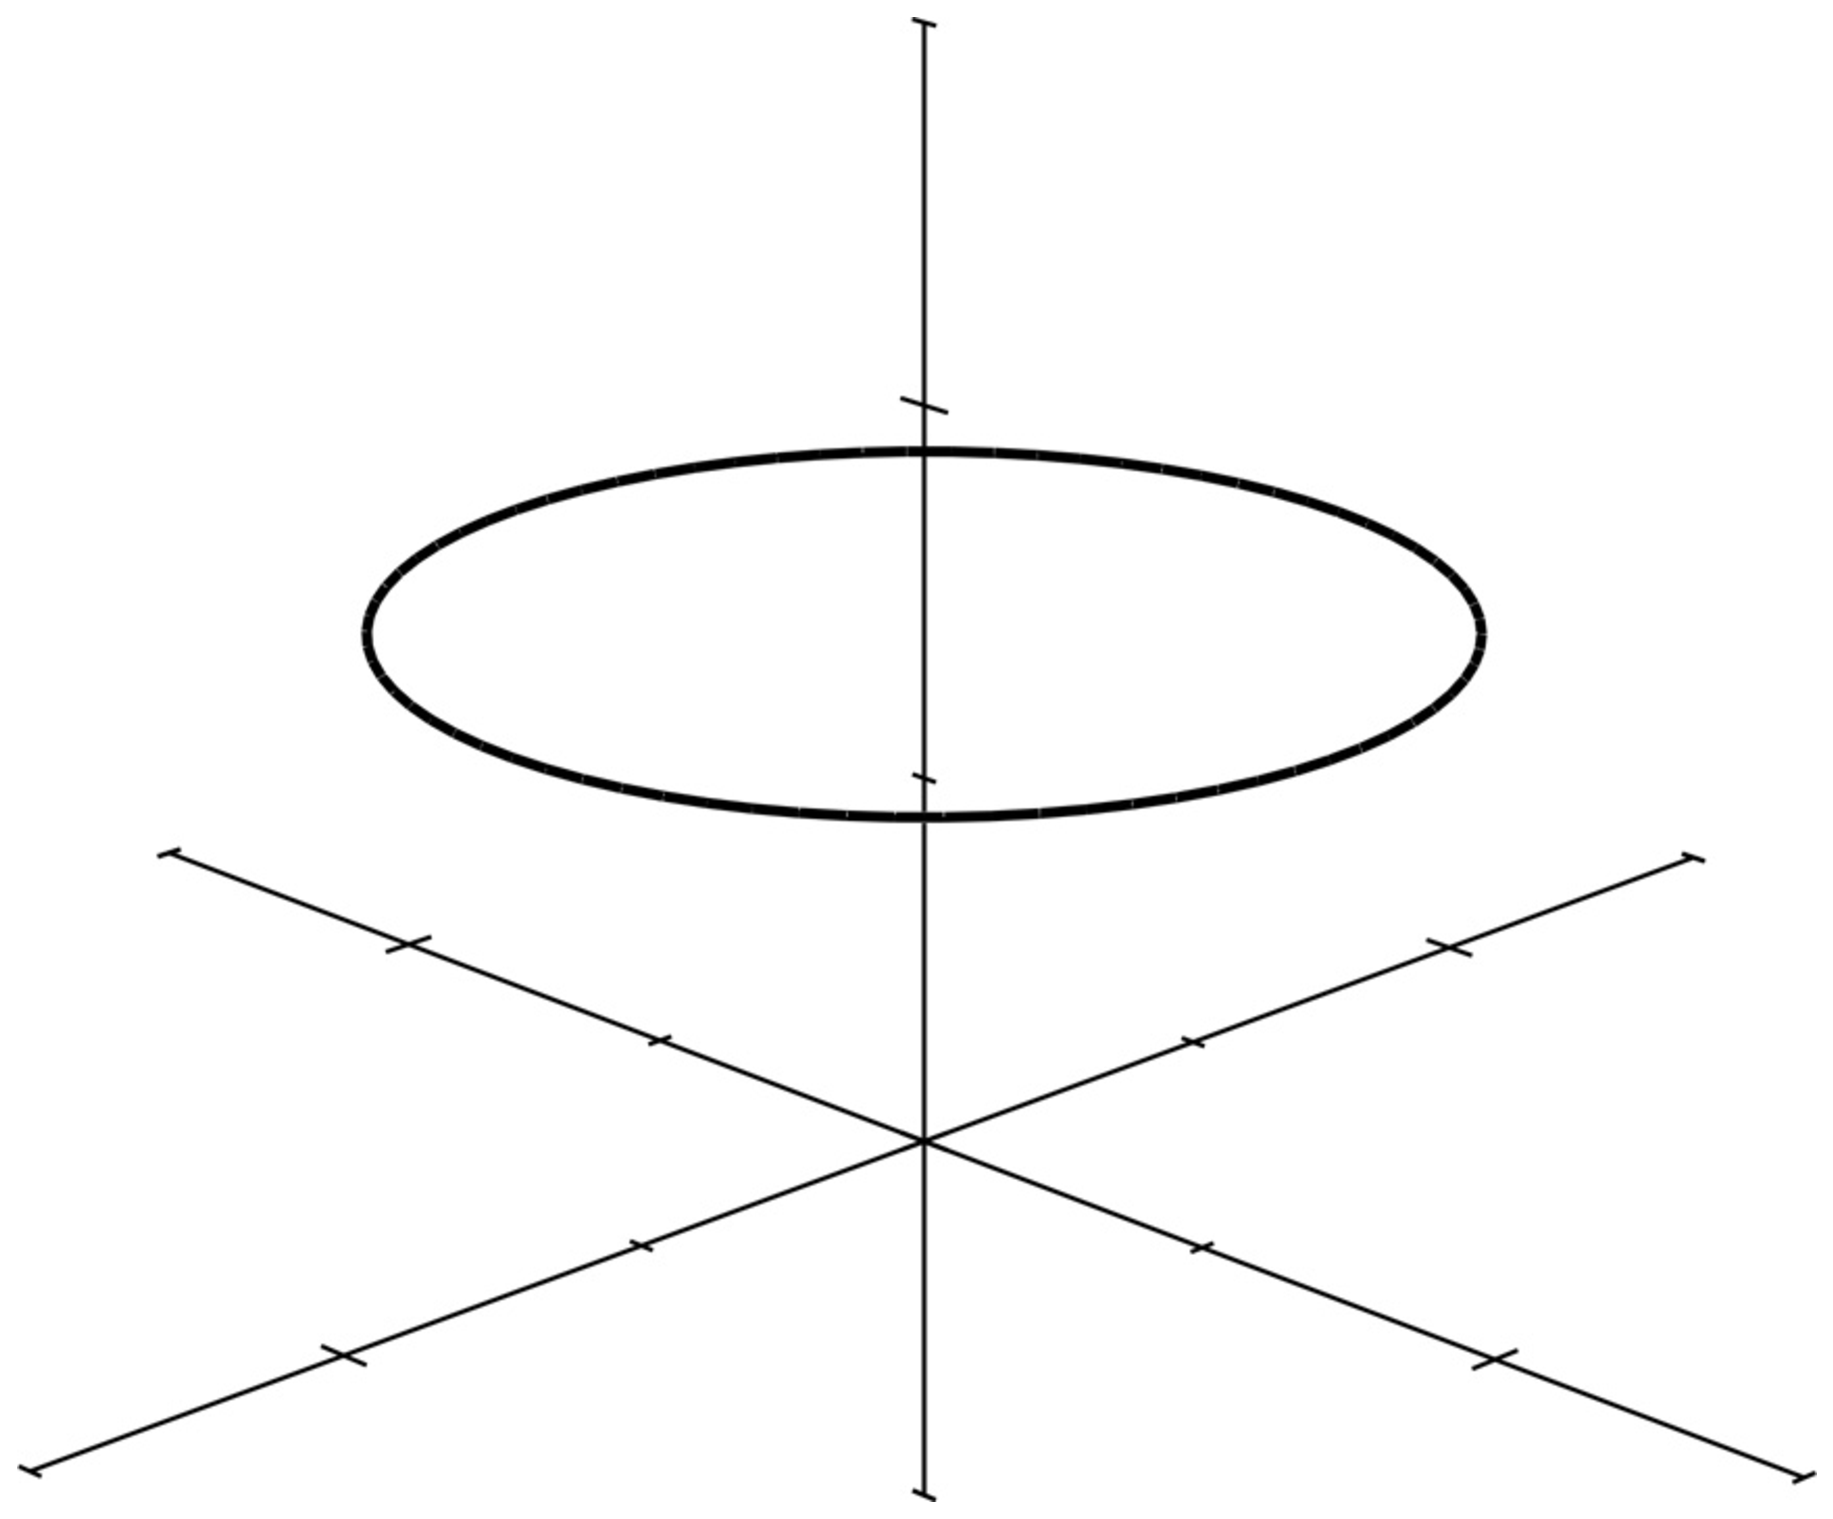
\includegraphics[width=.25\textwidth]{figures/rhoandphigiven.eps}};
\draw[red, ultra thick] (2,-0.9)--(3,0);
\node[right] at (1.9, -0.5){$\phi$};
\node at (2, 2.5){$z$};
\node at (4.5, -2){$y$};
\node at (-0.5, -2){$x$};
\end{tikzpicture}
\end{center}

Giving the third coordinate, $\theta $ completely specifies the point of interest. This is demonstrated in the following picture. If the latitude corresponds to $\phi $, then we can think of $\theta$ as the longitude. 

\begin{center}
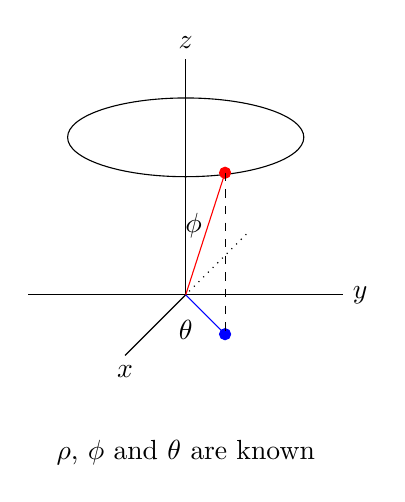
\begin{tikzpicture}
\draw(-1,-1,0)--(3,-1,0);
\draw(1,-1,0)--(1,2,0);
\draw[dotted](1,-1,-2)--(1,-1,0);
\draw(1,-1,0)--(1,-1,2);
\draw(1,1,0) circle [x radius=1.5cm, y radius=0.5cm];
\draw[red](1,-1,0)--(1.5,0.55,0);
\draw[fill, red](1.5,0.55,0) circle [radius=2pt];
\draw[blue](1,-1,0)--(1.5,-1.5,0);
\draw[fill,blue](1.5,-1.5,0) circle [radius=2pt];
\draw[dashed](1.5,0.55,0)--(1.5,-1.5,0);
\node[below] at (1,-1.2,0){$\theta$};
\node[right] at (3,-1,0){$y$};
\node[above] at (1,2,0){$z$};
\node[below] at (1,-1,2){$x$};
\node[above] at (1.1,-0.4,0){$\phi$};
%\node[right] at (1.4,0.1,0){$\rho$};
\node at (1, -3){$\rho$, $\phi$ and $\theta$ are known};
\end{tikzpicture}
\end{center}

The following picture summarizes the geometric meaning of the three coordinate systems. 

\begin{center}
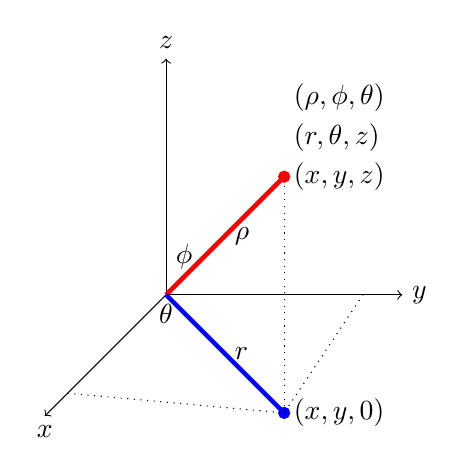
\begin{tikzpicture}
\draw[->](0,0,0)--(3,0,0);
\draw[->](0,0,0)--(0,3,0);
\draw[->](0,0,0)--(0,0,4);
\draw[ultra thick, red](0,0,0)--(1.5,1.5,0);
\draw[fill, red](1.5,1.5,0) circle [radius=2pt];
\draw[ultra thick, blue](0,0,0)--(1.5,-1.5,0);
\draw[fill, blue](1.5,-1.5,0) circle [radius=2pt];
\draw[dotted](-1.25,-1.25,0)--(1.5,-1.5,0)--(2.5,0,0);
\draw[dotted](1.5,-1.5,0)--(1.5,1.5,0);
\node[right] at (3,0,0){$y$};
\node[above] at (0,3,0){$z$};
\node[below] at (0,0,4){$x$};
\node[right] at (1.5,-1.5,0){$(x,y,0)$};
\node[below] at (0,0,0){$\theta$};
\node[above right] at (0,0.2,0){$\phi$};
\node[right] at (0.75,0.75,0){$\rho$};
\node[right] at (0.75,-0.75,0){$r$};
\node[right] at (1.5,1.5,0){$(x,y,z)$};
\node[right] at (1.5,2,0){$(r, \theta, z)$};
\node[right] at (1.5,2.5,0){$(\rho, \phi, \theta)$};
\end{tikzpicture}
\end{center}

Therefore, we can represent the same point in three ways, using Cartesian coordinates, $\left(x,y,z\right)$, cylindrical coordinates, $\left( r, \theta, z \right)$, and spherical coordinates $\left( \rho, \phi, \theta \right)$. 

Using this picture to review, call the point of interest $P$ for convenience. The Cartesian coordinates for $P$ are $(x,y,z)$. Then $\rho $ is the distance between the origin and the point $P$. The angle between
the positive $z$ axis and the line between the origin and $P$
 is denoted by $\phi $. Then $\theta $ is the angle
between the positive $x$ axis and the line joining the origin to the point 
$\left( x,y,0\right) $ as shown. This gives the spherical coordinates, $( \rho, \phi, \theta)$. Given the line from the origin to $\left( x,y,0\right) $,  $r=\rho \sin(\phi)$ is the length of this
line. Thus $r$ and $\theta $ determine a point in the $xy$-plane. In other words, $r$ and $\theta $ are the usual polar coordinates and $r\geq 0$ and $\theta \in \lbrack 0,2\pi )$. Letting $z$ denote the usual 
$z$ coordinate of a point in three dimensions, 
$\left( r,\theta ,z\right) $ are the cylindrical coordinates of $P$. 

The relation between spherical and cylindrical coordinates is that $r=\rho
\sin(\phi)$ and the $\theta$ is the same as the $\theta$ of cylindrical and polar
coordinates. 

We will now consider some examples.

\begin{example}{Describing a Surface in Spherical Coordinates}{}
Express the surface $z=\frac{1}{\sqrt{3}}\sqrt{x^{2}+y^{2}}$ in spherical
coordinates.
\end{example}

\begin{solution}
We will use the equations from above:
\[
\begin{array}{l}
x =\rho \sin \left( \phi \right) \cos \left( \theta \right), \phi \in 
\left[ 0,\pi \right]\\
 y =\rho \sin \left( \phi \right) \sin \left( \theta \right) ,\text{ }\theta
\in \lbrack 0,2\pi ) \\
 z =\rho \cos \phi \text{, }\rho \geq 0
\end{array}
\]

To express the surface in spherical coordinates, we substitute these expressions into the equation.  
This is done as follows:
\begin{equation*}
\rho \cos \left( \phi \right) =\frac{1}{\sqrt{3}}\sqrt{\left( \rho \sin
\left( \phi \right) \cos \left( \theta \right) \right) ^{2}+\left( \rho \sin
\left( \phi \right) \sin \left( \theta \right) \right) ^{2}}=\allowbreak 
\frac{1}{3}\sqrt{3}\rho \sin \left( \phi \right).
\end{equation*}
This reduces to 
\begin{equation*}
\tan \left( \phi \right)=\sqrt{3}
\end{equation*}
and so $\phi =\pi /3$.
\end{solution}

\begin{example}{Describing a Surface in Spherical Coordinates}{}
Express the surface $y=x$ in terms of spherical coordinates.
\end{example}

\begin{solution}
Using the same procedure as the previous example, this says $\allowbreak \rho \sin \left( \phi \right) \sin \left( \theta
\right) =\rho \sin \left( \phi \right) \cos \left( \theta \right)$. Simplifying,  $\sin \left( \theta \right) =\cos \left( \theta \right)$, which you could also write $\tan \left( \theta \right)=1$.
\end{solution}

We conclude this section with an example of how to describe a surface using cylindrical coordinates. 

\begin{example}{Describing a Surface in Cylindrical Coordinates}{}
Express the surface $x^{2}+y^{2}=4$ in cylindrical coordinates.
\end{example}

\begin{solution}
Recall that to convert from Cartesian to cylindrical coordinates, we can use the following equations:
\[
x =r\cos \left( \theta \right) , y=r\sin \left( \theta \right) , z =z
\]

Substituting these equations in for $x,y,z$ in the equation for the surface, we have  
\[
r^{2}\cos ^{2} \left( \theta \right) +r^{2}\sin ^{2} \left( \theta \right)=4
\]
This can be written as $r^2 ( \cos^{2} \left( \theta \right)+ \sin^{2} \left(\theta\right) ) = 4$. Recall that $ \cos^{2} \left( \theta \right)+ \sin^{2} \left( \theta \right)=1$.  Thus $r^{2} = 4$ or $r=2$.
\end{solution}